\documentclass[11pt]{article}
\usepackage[margin=1in]{geometry}
\usepackage{amsmath,amssymb,booktabs,graphicx,setspace,caption,hyperref}
\usepackage[T1]{fontenc}
\usepackage{mathpazo}
\setlength{\parindent}{0pt}
\setlength{\parskip}{0.6em}
\captionsetup{font=small,skip=6pt}
\title{Panel MS-AR(1) with quarterly seasonals, full sample\\[0.4em]\large Real GDP per worker (period-average USD)}
\author{}
\date{}
\begin{document}
\maketitle
\section{Model}
Joint panel Markov-switching AR(1) around a linear trend with quarterly seasonal means, three regimes:
\begin{align}
y_{it} &= a_i + g\, t + d_{2i} Q2_t + d_{3i} Q3_t + d_{4i} Q4_t + z_{it}, \\
z_{i,t+1} &= \bigl(1-\rho(s_{it})\bigr)\mu(s_{it}) + \rho(s_{it})\, z_{it} + \sigma(s_{it})\,\varepsilon_{it}, \\
s_{i,t+1} &\sim \Pi(\,\cdot\mid s_{it}).
\end{align}
Q1 is the omitted quarter (absorbed in $a_i$). Specification 1 sets $a_i\equiv a$ and $d_{ji}\equiv d_j$ (common dummies). Specification 2 keeps common $d_j$ and lets $a_i\sim\mathcal{N}(\alpha,\omega_a^2)$, integrating $a_i$ by 11-point Gauss--Hermite. Specification 3 lets $a_i\sim\mathcal{N}(\alpha,\omega_a^2)$ and $d_{ji}\sim\mathcal{N}(\delta_j,\omega_j^2)$ independently; the four-dimensional country integral is a Laplace approximation. The slope $g$ is common. $|\rho|<0.99$. Median $\mu$ pinned at 0. Cycles use posterior means (GH or Laplace mode). Standard errors are delta-method from a numerical Hessian on shared parameters.
\clearpage
\section{Common intercept, linear trend, and quarterly dummies}
2026-09-14 panel, full sample: log real GDP per worker. 90 countries, 8489 observations, 1963-Q1--2026-Q2. Fitted countries: 90. Observations: 8489. Log-likelihood: 13182.75. Ergodic mean of the cycle $E[z]=0.5738$ (0.0863).
Common intercept $a=-5.4283$ (0.1150). Common slope $g=-0.0004$ (0.0016). Seasonal dummies (Q1 omitted): $d_{Q2}=0.0161$ (0.0008), $d_{Q3}=0.0106$ (0.0009), $d_{Q4}=0.0432$ (0.0008).
\begin{table}[h]
\centering
\caption{Regime AR(1), transition matrix, and ergodic $\pi$. Columns are regimes.}
\begin{tabular}{lccc}
\toprule
 & (0) & (1) & (2) \\
\midrule
$\mu$ & -0.8032 & 0.0000 & 1.4857 \\
 & (0.3159) & --- & (0.0734) \\ \addlinespace
$\sigma$ & 0.1789 & 0.0660 & 0.0281 \\
 & (0.0049) & (0.0012) & (0.0004) \\ \addlinespace
$\rho$ & 0.9900 & 0.9900 & 0.9900 \\
 &  & (0.0000) & (0.0000) \\ \addlinespace
$\Pi_{0\cdot}$ & 0.9786 & 0.0171 & 0.0042 \\
 & (0.0060) & (0.0050) & (0.0030) \\ \addlinespace
$\Pi_{1\cdot}$ & 0.0040 & 0.9812 & 0.0148 \\
 & (0.0013) & (0.0028) & (0.0025) \\ \addlinespace
$\Pi_{2\cdot}$ & 0.0016 & 0.0138 & 0.9846 \\
 & (0.0012) & (0.0023) & (0.0021) \\ \addlinespace
$\pi$ & 0.1159 & 0.4351 & 0.4490 \\
 & (0.0248) & (0.0346) & (0.0362) \\ \addlinespace
\bottomrule
\end{tabular}
\end{table}
\begin{figure}[h]
\centering
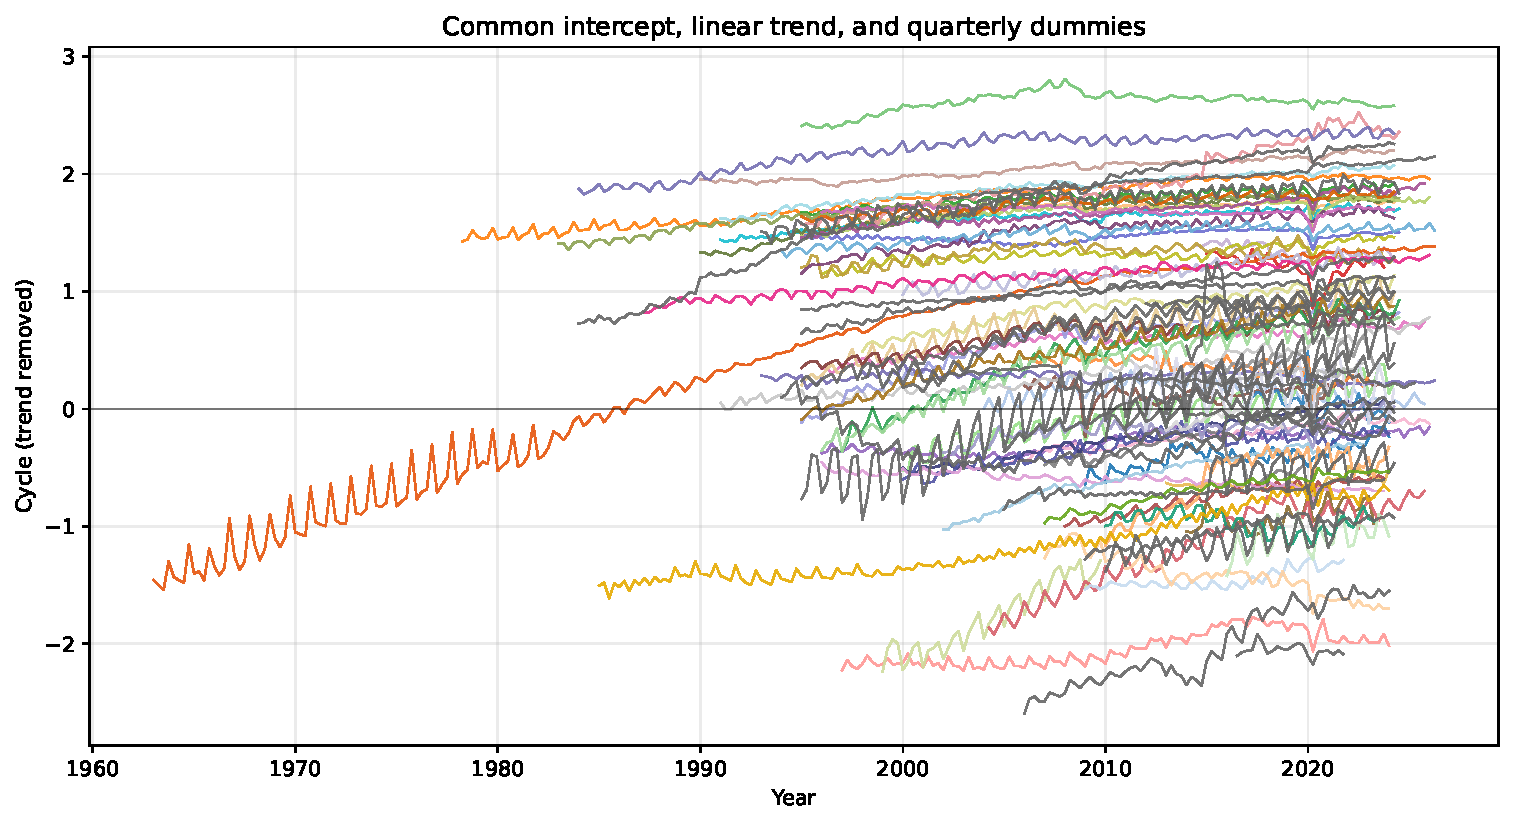
\includegraphics[width=0.75\textwidth]{figs/cycle_common_ag_q.pdf}
\caption{Country cycles after removing the linear trend and quarterly means.}
\end{figure}
\clearpage
\section{RE intercepts, common trend and quarterly dummies}
2026-09-14 panel, full sample: log real GDP per worker. 90 countries, 8489 observations, 1963-Q1--2026-Q2. Fitted countries: 90. Observations: 8489. Log-likelihood: 13468.95. Ergodic mean of the cycle $E[z]=0.1052$ (0.0486).
Random intercepts $a_i\sim N(\alpha,\omega^2)$ with $\alpha=-5.8735$ (0.0813), $\omega=0.7661$ (0.0181). Posterior-mean $a_i$: mean -6.133, min -8.144, max -4.436. Common slope $g=0.0179$ (0.0012). Seasonal dummies (Q1 omitted): $d_{Q2}=0.0160$ (0.0008), $d_{Q3}=0.0098$ (0.0009), $d_{Q4}=0.0420$ (0.0008).
\begin{table}[h]
\centering
\caption{Regime AR(1), transition matrix, and ergodic $\pi$. Columns are regimes.}
\begin{tabular}{lccc}
\toprule
 & (0) & (1) & (2) \\
\midrule
$\mu$ & -0.4259 & 0.0000 & 0.5050 \\
 & (0.0617) & --- & (0.0791) \\ \addlinespace
$\sigma$ & 0.1703 & 0.0662 & 0.0267 \\
 & (0.0049) & (0.0011) & (0.0004) \\ \addlinespace
$\rho$ & 0.6493 & 0.9790 & 0.9899 \\
 & (0.0411) & (0.0058) & (0.0002) \\ \addlinespace
$\Pi_{0\cdot}$ & 0.9851 & 0.0108 & 0.0041 \\
 & (0.0047) & (0.0040) & (0.0024) \\ \addlinespace
$\Pi_{1\cdot}$ & 0.0020 & 0.9815 & 0.0165 \\
 & (0.0010) & (0.0027) & (0.0026) \\ \addlinespace
$\Pi_{2\cdot}$ & 0.0008 & 0.0154 & 0.9838 \\
 & (0.0007) & (0.0022) & (0.0022) \\ \addlinespace
$\pi$ & 0.0831 & 0.4436 & 0.4733 \\
 & (0.0226) & (0.0354) & (0.0365) \\ \addlinespace
\bottomrule
\end{tabular}
\end{table}
\begin{figure}[h]
\centering
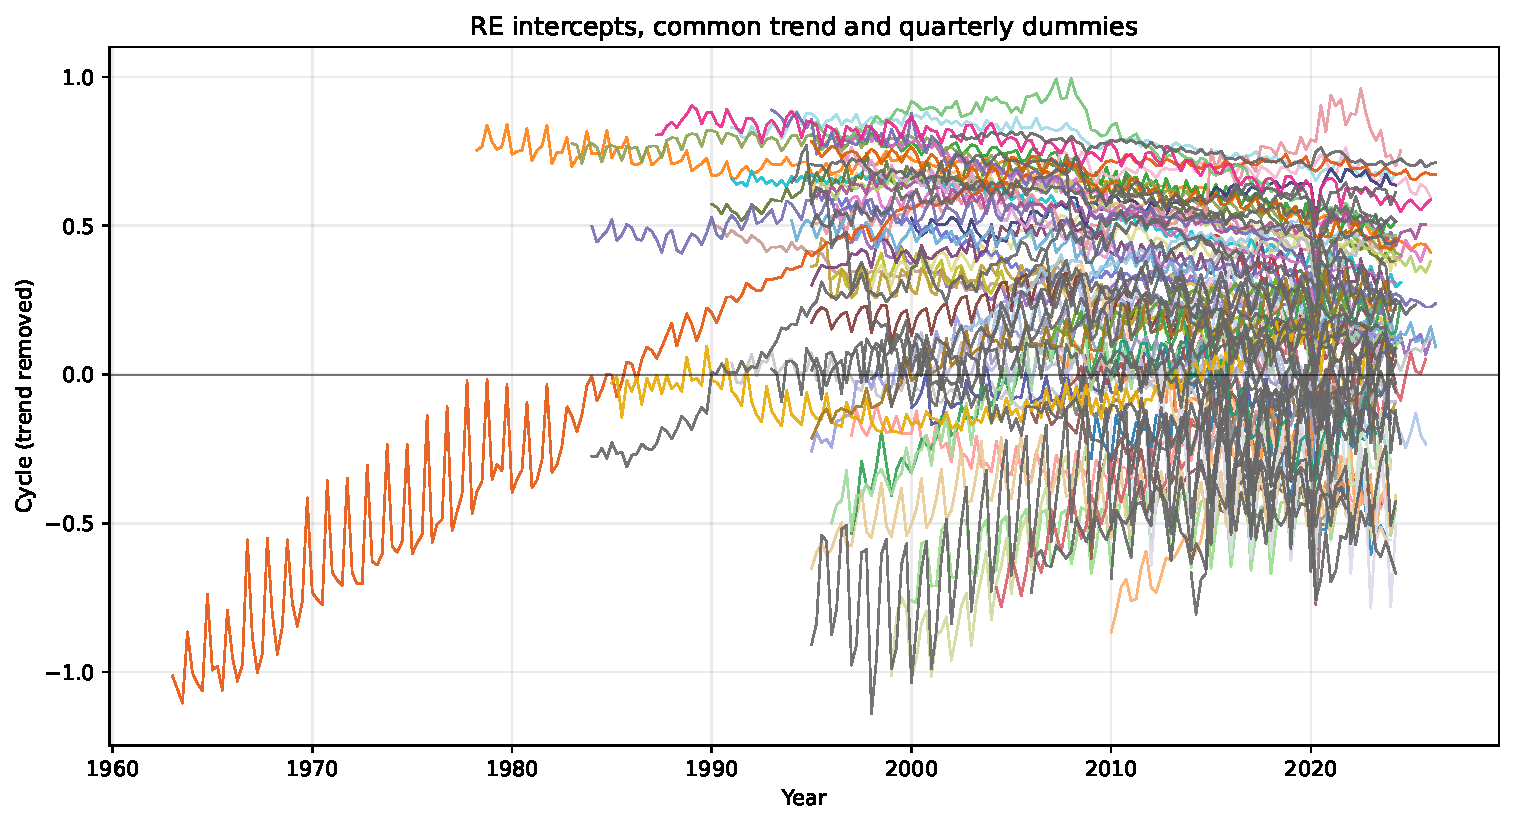
\includegraphics[width=0.75\textwidth]{figs/cycle_re_ai_q.pdf}
\caption{Country cycles after removing the linear trend and quarterly means.}
\end{figure}
\clearpage
\section{RE intercepts and RE quarterly effects (Laplace)}
2026-09-14 panel, full sample: log real GDP per worker. 90 countries, 8489 observations, 1963-Q1--2026-Q2. Fitted countries: 90. Observations: 8489. Log-likelihood: 13004.58. Ergodic mean of the cycle $E[z]=0.0245$ (0.0134).
Random intercepts $a_i\sim N(\alpha,\omega^2)$ with $\alpha=-5.9012$, $\omega=1.3492$. Posterior-mean $a_i$: mean -5.719, min -8.334, max -3.513. Common slope $g=0.0143$. Random quarterly effects $d_{ji}\sim N(\delta_j,\omega_j^2)$ (Q1 omitted): $\delta_{Q2}=-0.0499$, $\omega_{2}=0.0473$; $\delta_{Q3}=-0.1018$, $\omega_{3}=0.0761$; $\delta_{Q4}=-0.0669$, $\omega_{4}=0.0674$.
\begin{table}[h]
\centering
\caption{Regime AR(1), transition matrix, and ergodic $\pi$. Columns are regimes.}
\begin{tabular}{lccc}
\toprule
 & (0) & (1) & (2) \\
\midrule
$\mu$ & -1.3890 & 0.0000 & 1.0431 \\
 &  & --- &  \\ \addlinespace
$\sigma$ & 0.7501 & 0.0439 & 0.7492 \\
 &  &  &  \\ \addlinespace
$\rho$ & 0.8203 & 0.8616 & 0.8206 \\
 & (0.0048) & (0.0001) &  \\ \addlinespace
$\Pi_{0\cdot}$ & 0.8589 & 0.0667 & 0.0744 \\
 & (0.0043) & (0.0020) & (0.0023) \\ \addlinespace
$\Pi_{1\cdot}$ & 0.0408 & 0.9069 & 0.0523 \\
 & (0.0006) & (0.0014) & (0.0008) \\ \addlinespace
$\Pi_{2\cdot}$ & 0.0538 & 0.0559 & 0.8903 \\
 & (0.0009) & (0.0009) & (0.0012) \\ \addlinespace
$\pi$ & 0.2498 & 0.3933 & 0.3569 \\
 & (0.0062) & (0.0052) & (0.0044) \\ \addlinespace
\bottomrule
\end{tabular}
\end{table}
\begin{figure}[h]
\centering
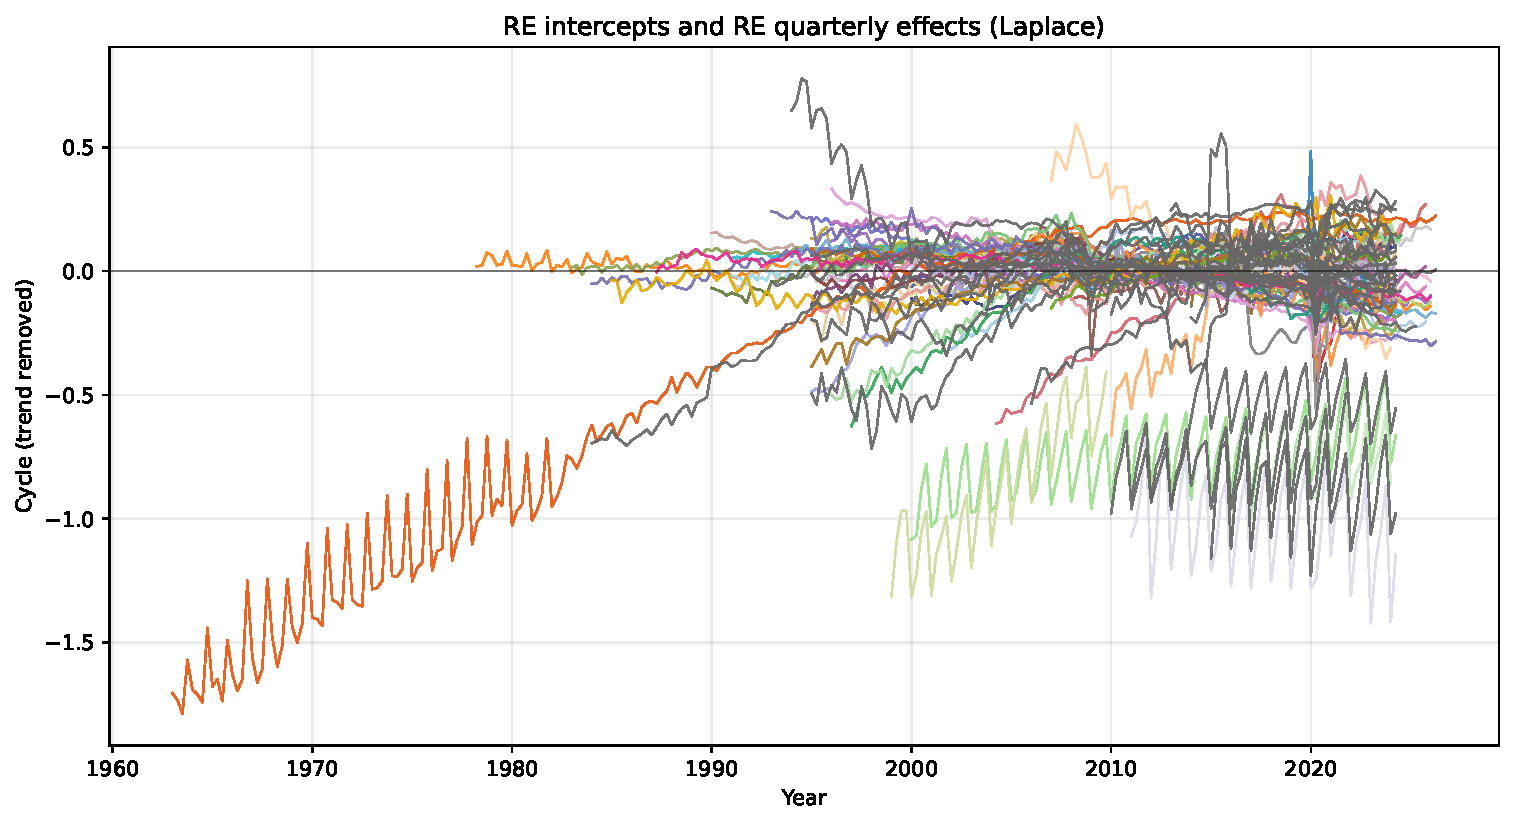
\includegraphics[width=0.75\textwidth]{figs/cycle_re_ai_qre.pdf}
\caption{Country cycles after removing the linear trend and quarterly means.}
\end{figure}
\end{document}
